\chapter{Introdução}

\section{Enquadramento\label{se:enquadramento}}
Esta dissertação encontra-se no âmbito do projeto \href{https://traderes.eu/}{TradeRES}, que estuda um sistema de mercado elétrico capaz de atender às necessidades da sociedade num sistema quase totalmente renovável. Tendo as características para se integrar nos \href{https://ods.pt/ods/}{ODS} \ref{fig:ODS}. \\
O estudo da acessibilidade das energias renováveis ao mercado vigente integra-se nos ODS n.º7, “Energia Renováveis e Acessíveis”, indo directamente de encontro a um dos pontos deste objectivo: 7.2.1 “Peso das energias renováveis no consumo total final de energia”. Por meio deste objectivo, a participação das renováveis no mercado faz também cumprir, embora indiretamente, o objectivo nº8 “Trabalho Digno e Crescimento Económico”, através do ponto 8.4, onde é dada primazia à eficiência dos recursos globais no consumo e na produção. Indiretamente, pois, ao haver um melhor uso das renováveis, o uso de energias não limpas vai diminuir, melhorando a gestão de recursos, e baixando o consumo de recursos naturais não renováveis. \\
Por último podemos incluir o objectivo n.º13, “Acção Climática”, no qual, referimos de novo a diminuição de consumo de recursos finitos, mas mais importante, a melhor gestão de recursos renováveis. Promovendo o planeamento e estratégias de combate a emissões de gases de efeito estufa. \\

\begin{figure}[h]
    \centering
    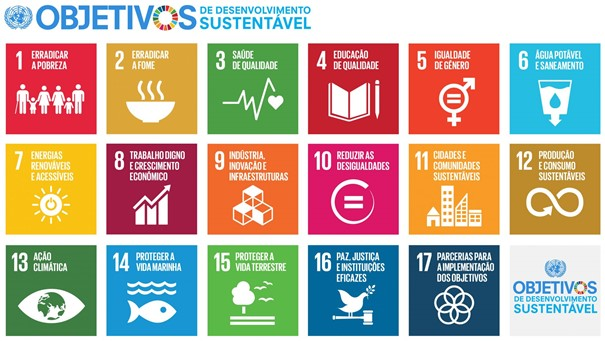
\includegraphics{Imagens/DesenvolvimentoSustentavel.jpg}
    \caption{Objectivos de Desenvolvimento Sustentável da ONU}
    \label{fig:ODS}
\end{figure}

\section{Objetivos e Perguntas de Pesquisa\label{se:objetivos}}

Foram aprovadas a nível europeu (2020) medidas de alteração aos serviços de sistema, que serão seguidas pelos Estados-Membros. Nesta dissertação, será realizada a aplicação dessas medidas, identificando as melhorias em relação ao design atual e avaliando se as novas medidas serão suficientes para garantir a operação de um sistema elétrico 100 renovável, potencialmente identificando ações adicionais para garantir a robustez e segurança do sistema elétrico sem o uso de combustíveis fósseis. \\

As seguintes perguntas guiarão esta pesquisa.\\

\begin{enumerate}[label=\alph*)]
  \item É positivo para as vRES participar no mercado de reserva?
  \item Como configurar essa participação para otimizar o lucro do ponto de vista das vRES?
  \item Essa participação é positiva para o sistema eléctrico num todo?
\end{enumerate}

Para responder a essas perguntas, utilizaremos dados de previsão de geração de energia renovável para estimar a energia necessária para alocação secundária. Atualmente, os valores de previsão desse mercado estão distantes do consumo real, o que resulta em alocações no dia anterior que não estão em conformidade com as necessidades reais. O objetivo deste trabalho é investigar se podemos obter previsões mais precisas da energia necessária utilizando técnicas de \textit{Machine Learning} (Aprendizado de Máquina). Isso possibilitará uma melhor gestão das alocações, resultando em um menor gasto de recursos energéticos e financeiros.

\section{Organização do Documento \label{se:organização}}

Este documento está divido em capitulos. Sendo que os primeiros apresentam uma introdução às ideias e temas \ref{ch:intro}, o estado de arte do temas na literatura publicada \ref{ch:revisao}, e por fim uma contextualização dos temas abordados \ref{ch:contexto}. \\
Segue um capitulo de explicação dos dados usado \ref{ch:dados}, onde se apresentam os mesmos juntamente com alguns estudos preliminares para compreender a naturuza e qualidades dos mesmos. \\
%TODO: adicinar onde os buscar e que estudos

O capitulo seguinte entra no ambito experimental da dissertação, onde se apresenta as diferentes arquitecturas \ref{ch:arch} utilizadas, incluindo uma explicação dos componentes das mesmas. \\

Os capítulos 6 e 7 são bastatante paralelos, sendo que o sexto \ref{ch:metodos} apresenta a metologia do trabalho, e explica todas as experiências, e o sétimo \ref{ch:resultados_discussao} apresenta apenas os resultados e conclusoes experiência a experiência. \\

Termina com um capitulo conclusivo \ref{ch:conclusao} onde são avaliadas as experiências como um todo, e o seu impacto no ambito dos mercados de reserva. \\

